\setAuthor{Mihkel Kree}
\setRound{piirkonnavoor}
\setYear{2006}
\setNumber{G 6}
\setDifficulty{4}
\setTopic{Geomeetriline optika}

\prob{Biprisma}
Paralleelne kiirtekimp langeb võrdhaarsele kolmnurksele prismale risti prisma tahuga (vt joonist). Prisma teravnurgad on väikesed, suurusega $\alpha$. Prisma materjali murdumisnäitaja on $n$. Prismast kaugusel $d$ paikneb koondav lääts fookuskaugusega $f$. Läätse optiline peatelg on paralleelne kiirtekimbu esialgse sihiga ning läbib prisma tipunurka. Missugune pilt tekib läätse fokaaltasandis asuvale ekraanile? Leida pilti iseloomustavad parameetrid. Kuidas sõltub pilt kaugusest $d$? 

\emph{Märkus:} väikeste nurkade korral kehtib lähendus $\tan \alpha \approx \sin \alpha \approx \alpha$.

\begin{center}
	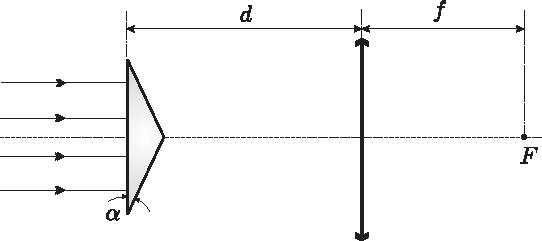
\includegraphics[width=\linewidth]{2006-v2g-06-yl}
\end{center}

\hint
Valguskiir siseneb prismasse murdumata, sest kiir on normaali sihiline. Küll aga toimub murdumine prismast väljudes. Kuna terve tahu ulatuses on langemisnurk sama, tekitab üks tahk paralleelse kiirtekimbu. Kuna meil on kaks murdvat tahku, on esialgne kiirtekimp pärast prisma läbimist jagunenud kaheks.

\solu
Valguskiir siseneb prismasse murdumata, sest kiir on normaali sihiline. Küll aga toimub murdumine prismast väljudes. Kuna terve tahu ulatuses on langemisnurk sama, tekitab üks tahk paralleelse kiirtekimbu (vt joonist). Kuna meil on kaks murdvat tahku, on esialgne kiirtekimp pärast prisma läbimist jagunenud kaheks.

On lihtne märgata, et langemisnurk, millega kiired langevad murdvale tahule, on $\alpha$. 
Vastavalt murdumisseadusele saame murdumisnurga $\gamma$ jaoks seose:
\[
\sin \gamma = n \sin \alpha.
\]
Väikeste nurkade jaoks lihtsustub see avaldis: $\gamma = n\alpha$. Kiir kaldus seega oma esialgsest sihist kõrvale nurga
\[
\beta = \gamma - \alpha = (n - 1) \alpha
\]
võrra. 

Teame, et paralleelne kiirtekimp koondub kumerläätse fokaaltasandis. Seega tekib fokaaltasandis asuvale ekraanile sümmeetriliselt kaks valgustäppi, teine teisele poole optilist peatelge. Arvutame ka nende kaugused peateljest. Selleks kasutame läbi läätse keskpunkti tõmmatud kiirt, mis asetseb peateljega nurga $\beta$ all. Täisnurksest kolmnurgast saame valguspunkti kauguse peateljest:
\[
s = f \tan \beta \approx f \beta = (n - 1)\alpha f.
\]
Ilmselt ei sõltu ekraanil tekkiv pilt kaugusest $d$.

Et olla päris täpne, tuleks siiski märkida, et $d$ kasvades piisavalt suureks hakkavad täpid muutuma tuhmimaks, kuni lõpuks kaovad üldse, sest siis kiired enam läätse ei läbi.

\begin{center}
	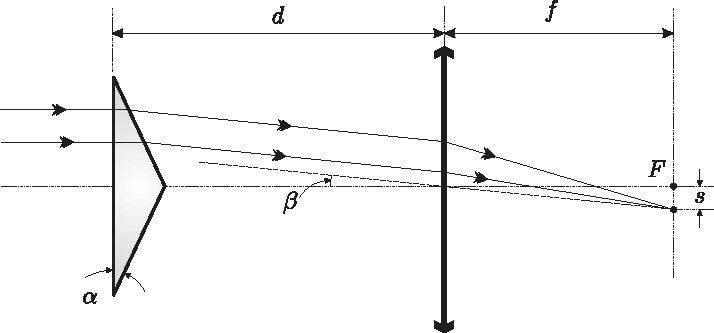
\includegraphics[width=\linewidth]{2006-v2g-06-lah}
\end{center}
\probend